
\documentclass[11pt]{article}

%%%%%%%%%%%%
% Packages %
%%%%%%%%%%%%
\usepackage[dvipsnames]{xcolor}
\hyphenpenalty=10000
\usepackage{tikz}
\usetikzlibrary{shapes,arrows}

\usepackage{tocloft}
\renewcommand\cftsecleader{\cftdotfill{\cftdotsep}}
\def\undertilde#1{\mathord{\vtop{\ialign{##\crcr
$\hfil\displaystyle{#1}\hfil$\crcr\noalign{\kern1.5pt\nointerlineskip}
$\hfil\tilde{}\hfil$\crcr\noalign{\kern1.5pt}}}}}
\usepackage{cleveref}
\usepackage{xcolor}
\usepackage[colorlinks = true,
            linkcolor = black,
            urlcolor  = blue,
            citecolor = black,
            anchorcolor = black]{hyperref}
\usepackage{epstopdf}
\usepackage{braket}
\usepackage{upgreek}
\usepackage{caption}
\usepackage{booktabs}
\usepackage{subcaption}
\usepackage{amssymb,latexsym,amsmath,gensymb}
\usepackage{latexsym}
\usepackage{graphicx}
\usepackage{float}
\usepackage{enumitem}
\usepackage{pdflscape}
\usepackage{url}
\usepackage{array}
\newcolumntype{C}{>{$\displaystyle} c <{$}}
\usepackage{tikz, calc}
\usetikzlibrary{shapes.geometric, arrows, calc}
\tikzstyle{norm} = [rectangle, rounded corners, minimum width=2cm, minimum height=1cm,text centered, draw=black]
\tikzstyle{arrow} = [thick, ->, >=stealth]

\newcommand{\argmin}{\arg\!\min}
\newcommand{\me}{\mathrm{e}}
\providecommand{\e}[1]{\ensuremath{\times 10^{#1}}} 
\providecommand{\mb}[1]{\mathbf{#1}}
\providecommand{\mf}[1]{\mathbf{#1}}
\providecommand{\ro}[1]{\mathbf{\mathbf{r}}_o}
\providecommand{\so}[1]{\mathbf{\hat{s}}_o}
\providecommand{\rb}[1]{\mathbf{r}_b}
\providecommand{\rbm}[1]{r_b^{\text{m}}}
\providecommand{\rd}[1]{\mathbf{r}_d}
\providecommand{\mh}[1]{\mathbf{\hat{#1}}}
\providecommand{\bs}[1]{\boldsymbol{#1}} 
\providecommand{\intinf}{\int_{-\infty}^{\infty}}
\providecommand{\fig}[4]{
  % filename, width, caption, label
\begin{figure}[h]
 \captionsetup{width=1.0\linewidth}
 \centering
 \includegraphics[width = #2\textwidth]{#1}
 \caption{#3}
 \label{fig:#4}
\end{figure}
}

\makeatletter
\renewcommand*\env@matrix[1][*\c@MaxMatrixCols c]{%
  \hskip -\arraycolsep
  \let\@ifnextchar\new@ifnextchar
  \array{#1}}
\makeatother

\newcommand{\tensor}[1]{\overset{\text{\tiny$\leftrightarrow$}}{\mb{#1}}}
\newcommand{\tunderbrace}[2]{\underbrace{#1}_{\textstyle#2}}
\providecommand{\figs}[7]{
  % filename1, filename2, caption1, caption2, label1, label2, shift
\begin{figure}[H]
\centering
\begin{minipage}[b]{.45\textwidth}
  \centering
  \includegraphics[width=1.0\linewidth]{#1}
  \captionsetup{justification=justified, singlelinecheck=true}
  \caption{#3}
  \label{fig:#5}
\end{minipage}
\hspace{2em}
\begin{minipage}[b]{.45\textwidth}
  \centering
  \includegraphics[width=1.0\linewidth]{#2}
  \vspace{#7em}
  \captionsetup{justification=justified}
  \caption{#4}
  \label{fig:#6}
\end{minipage}
\end{figure}
}
\makeatletter

\providecommand{\code}[1]{
\begin{center}
\lstinputlisting{#1}
\end{center}
}

\newcommand{\crefrangeconjunction}{--}
%%%%%%%%%%%
% Spacing %
%%%%%%%%%%%
% Margins
\usepackage[
top    = 1.5cm,
bottom = 1.5cm,
left   = 1.5cm,
right  = 1.5cm]{geometry}

% Indents, paragraph space
%\usepackage{parskip}
\setlength{\parskip}{1.5ex}

% Section spacing
\usepackage{titlesec}
\titlespacing*{\title}
{0pt}{0ex}{0ex}
\titlespacing*{\section}
{0pt}{0ex}{0ex}
\titlespacing*{\subsection}
{0pt}{0ex}{0ex}
\titlespacing*{\subsubsection}
{0pt}{0ex}{0ex}

% Line spacing
\linespread{1.1}

%%%%%%%%%%%%
% Document %
%%%%%%%%%%%%
\begin{document}
\title{\vspace{-2.5em} Spatio-angular transfer functions for polarized fluorescence microscopes\vspace{-1em}}  \author{Talon Chandler, Min Guo, Hari Shroff, Rudolf Oldenbourg, Patrick La Rivi\`ere}
\date{\vspace{-1em}\today\vspace{-1em}}
\maketitle
\section{Introduction}
These notes are a continuation of the
\href{https://github.com/talonchandler/polharmonic/blob/master/notes/2018-02-23-spatio-angular-kernel/report/report.pdf}{2018-02-23
  notes} on the spatio-angular transfer functions for unpolarized fluorescence
microscopes. We will use the same notation and extend those results to microscopes
with polarized illumination and detection.

\section{Polarized illumination}
We can model polarized excitation using a spatio-angular excitation point
response function $h_{\text{exc}}(\ro{}, \so{})$. In these notes we will only
consider spatially uniform excitation patterns $h_{\text{exc}}(\so{})$, but we
would need the full function to model structured illumination patterns.

We calculated several spatio-angular excitation point response functions in our
Optics Express paper \cite{chandler17} (in the paper we called this function the
excitation efficiency for a single dipole, but this is equivalent to the
excitation point spread function). If we place a spatially incoherent and
spatially uniform light source (or its image) in the aperture plane with the
optical axis along the $\mh{z}$ axis, then the excitation point response function
is given by
\begin{align}
  h^{\mh{z}}_{\text{exc}}(\Theta, \Phi; \phi_{\text{exc}}) &= \bar{D}\{\bar{A} + \bar{B}\sin^{2}{\Theta} + \bar{C}\sin^{2}{\Theta} \cos{[2 (\Phi - \phi_{\text{exc}}})]\}\label{eq:scalarabs},
\end{align}
where
$\so{} = \cos\Phi\sin\Theta\mh{x} + \sin\Phi\sin\Theta\mh{y} + \cos\Theta\mh{z}$,
the illumination polarizer orientation is given by $\mh{p} = \cos\phi_{\text{exc}}\mh{x} + \sin\phi_{\text{exc}}\mh{y}$, and 
\begin{subequations}
\begin{align}
  \bar{A} &= \frac{1}{4} - \frac{3}{8} \cos{\alpha } + \frac{1}{8} \cos^{3}{\alpha },\\
  \bar{B} &= \frac{3}{16} \cos{\alpha } - \frac{3}{16} \cos^{3}{\alpha },\\
  \bar{C} &= \frac{7}{32} - \frac{3}{32} \cos{\alpha } - \frac{3}{32} \cos^{2}{\alpha } - \frac{1}{32} \cos^{3}{\alpha},\\
  \bar{D} &= \frac{4}{3(1 - \cos\alpha)},
\end{align}\label{eq:coefficients}%
\end{subequations}
where $\alpha = \arcsin(\text{NA}/n_o)$. I'm using bars on the constants to
avoid notation overlap with the previous note set. We can rewrite this
expression in terms of spherical harmonics as
\begin{align}
  h^{\mh{z}}_{\text{exc}}(\so{}; \mh{p}) \propto\, &[2\bar{A} + (4/3)\bar{B}]\bar{D}y_0^0(\so{}) - \frac{4\sqrt{5}}{15}\bar{B}\bar{D}y_2^0(\so{}) + \nonumber\\ &\frac{4\bar{C}\bar{D}}{\sqrt{15}}\left\{[(\mh{p}\cdot\mh{x})^2 - (\mh{p}\cdot\mh{y})^2]y_2^2(\so{}) - 2(\mh{p}\cdot\mh{x})(\mh{p}\cdot\mh{y})y_2^{-2}(\so{})\right\}. \label{eq:genpsf}
\end{align}
We can simplify this result further by redefining the constants and normalizing
\begin{align}
  h^{\mh{z}}_{\text{exc}}(\so{}; \mh{p}) &= y_0^0(\so{}) - \frac{1}{\sqrt{5}}\tilde{A}y_2^0(\so{}) + \sqrt{\frac{3}{5}}\tilde{B}\left\{[(\mh{p}\cdot\mh{x})^2 - (\mh{p}\cdot\mh{y})^2]y_2^2(\so{}) - 2(\mh{p}\cdot\mh{x})(\mh{p}\cdot\mh{y})y_2^{-2}(\so{})\right\}, \label{eq:genpsf}
\end{align}
where
\begin{subequations}
\begin{align}
  \tilde{A} &\equiv \cos^2(\alpha/2)\cos(\alpha),\\
  \tilde{B} &\equiv \frac{1}{12}(\cos^2\alpha + 4\cos\alpha + 7).
\end{align}\label{eq:coefficients}%
\end{subequations}

The light-sheet excitation point response function is given by Eq.
\ref{eq:genpsf} in the limit of small NA ($\tilde{A} \rightarrow 1$ and $\tilde{B} \rightarrow 1$) which gives
\begin{align}
  h^{\mh{z}, \text{ls}}_{\text{exc}}(\so{}; \mh{p}) \equiv \lim_{\alpha \rightarrow 0} h^{\mh{z}}_{\text{exc}}(\so{}) = y_0^0(\so{}) - \frac{1}{\sqrt{5}}y_2^0(\so{}) + \sqrt{\frac{3}{5}}\left\{[(\mh{p}\cdot\mh{x})^2 - (\mh{p}\cdot\mh{y})^2]y_2^2(\so{}) - 2(\mh{p}\cdot\mh{x})(\mh{p}\cdot\mh{y})y_2^{-2}(\so{})\right\}.
\end{align}
To find the excitation point response function for illumination along the
$\mh{x}$ axis we need to change every $\mh{x}$ and $\mh{y}$ to $\mh{z}$ and
$-\mh{y}$, respectively. Rotating the spherical harmonics is not trivial,
but we show the relevant transformation matrix in Appendix \ref{sec:sh}. The
excitation point response function for illumination along the $\mh{x}$ axis is
given by
\begin{align}
  h^{\mh{x}, \text{ls}}_{\text{exc}}(\so{}; \mh{p}) = y_0^0(\so{}) - \frac{1}{\sqrt{5}}y_2^0(\so{}) + \sqrt{\frac{3}{5}}\left\{[(\mh{p}\cdot\mh{z})^2 - (\mh{p}\cdot\mh{y})^2]\left[\frac{\sqrt{3}}{2}y_2^0(\so{}) + \frac{1}{2}y_2^2(\so{})\right] + 2(\mh{p}\cdot\mh{z})(\mh{p}\cdot\mh{y})y_2^{-1}(\so{})\right\}.
\end{align}

To find the excitation transfer functions we need to calculate
\begin{align}
  H_{l, \text{exc}}^m = \int_{\mathbb{S}^2} d\so{}\, h_{\text{exc}}(\so{}) y_l^m(\so{}).
\end{align}
This calculation is straightforward now that we've expressed the excitation
point response functions in terms of spherical harmonics. The excitation
transfer functions are
\begin{align}
  H^{m,\mh{z}}_{l,\text{exc}}(\mh{p}) &= \delta(l, m) - \frac{1}{\sqrt{5}}\tilde{A}\delta(l-2, m)(\so{}) + \sqrt{\frac{3}{5}}\left\{[(\mh{p}\cdot\mh{x})^2 - (\mh{p}\cdot\mh{y})^2]\delta(l-2, m-2) - 2(\mh{p}\cdot\mh{x})(\mh{p}\cdot\mh{y})\delta(l-2, m+2)\right\},\\
  H^{m,\mh{z}, \text{ls}}_{l,\text{exc}}(\mh{p}) &= \delta(l,m) - \frac{1}{\sqrt{5}}\delta(l-2, m) + \sqrt{\frac{3}{5}}\left\{[(\mh{p}\cdot\mh{x})^2 - (\mh{p}\cdot\mh{y})^2]\delta(l-2,m-2) - 2(\mh{p}\cdot\mh{x})(\mh{p}\cdot\mh{y})\delta(l-2, m+2)\right\},\\
  H^{m,\mh{x}, \text{ls}}_{l, \text{exc}}(\mh{p}) &= \delta(l,m) - \frac{1}{\sqrt{5}}\delta(l-2, m) + \sqrt{\frac{3}{5}}\Bigg\{[(\mh{p}\cdot\mh{z})^2 - (\mh{p}\cdot\mh{y})^2]\left[\frac{\sqrt{3}}{2}\delta(l-2,m) + \frac{1}{2}\delta(l-2, m-2)\right]\nonumber\\ &\hspace{20em}+ 2(\mh{p}\cdot\mh{z})(\mh{p}\cdot\mh{y})\delta(l-2, m+1)\Bigg\}.     \end{align}

\section{Polarized detection}
In the previous note set we found the spatio-angular detection point spread
function for unpolarized fluorescence microscopes. In this section we will find
the spatio-angular detection point spread function when there is a linear
polarizer in the detection path.

The electric field in the back-focal plane of a fluorescence microscope under
the paraxial approximation is given by
\begin{align}
   \mb{\tilde{e}}^{(p)}_b(\rb{};\ro{}, \so{}) \propto
  \begin{bmatrix}
    y_1^1(\so{}) -\frac{2r_b}{f_o}\cos\phi_by_1^0(\so{})\\
    y_1^{-1}(\so{}) -\frac{2r_b}{f_o}\sin\phi_by_1^0(\so{})\\
    0
  \end{bmatrix}.\label{eq:bfp}
\end{align}
In these notes we will ignore the phase term in the back focal plane---see the
previous notes for more details on shift invariance. Alternatively, we can say
that Eq. \ref{eq:bfp} is the electric field in the back focal plane created by a
single dipole at the focal point of the objective.

If we place a polarizer oriented along $\mh{p}_d$ in the back focal plane then
the electric field becomes
\begin{align}
   \mb{\tilde{e}}^{(p)}_b(\rb{};\ro{}, \so{}) \propto \mh{p}_d \cdot
  \begin{bmatrix}
    y_1^1(\so{}) -\frac{2r_b}{f_o}\cos\phi_by_1^0(\so{})\\
    y_1^{-1}(\so{}) -\frac{2r_b}{f_o}\sin\phi_by_1^0(\so{})\\
    0
  \end{bmatrix}.
\end{align}
To find the electric field in the detector plane we need to take the
two-dimensional Fourier transform of each component. The dot product with the
polarizer is linear, so we can pull the Fourier transform inside and use the same
result from the previous notes
\begin{align}
  \tilde{\mb{e}}'^{(p)}_d(\ro{}', \so{}; \mh{p}_d) &\propto \mh{p}_d \cdot
  \begin{bmatrix}
    a^{(p)}(r_o')y_1^{1}(\so{}) + 2ib^{(p)}(r_o')\cos\phi_o'y_1^{0}(\so{})\\
    a^{(p)}(r_o')y_1^{-1}(\so{}) + 2ib^{(p)}(r_o')\sin\phi_o'y_1^{0}(\so{})\\
    0\\
  \end{bmatrix}\label{eq:paracsf}. 
\end{align}
Finally, we can find the spatio-angular point spread function by taking the
squared modulus of the electric field on the detector
\begin{align}
  h'^{(p)}(\ro{}', \so{}; \mh{p}_d) &\equiv |\tilde{\mb{e}}'^{(p)}_d(\ro{}', \so{}; \mh{p}_d)|^2.
\end{align}
Expanding, factoring, and normalizing the result gives   
\begin{align}
    h'^{(p)}(\ro{}', \so{}; \mh{p}_d) &= {h'}_0^{0(p)}(\ro{}')y_0^0(\so{}) + {h'}_2^{0(p)}(\ro{}')y_2^0(\so{}) + {h'}_2^{2(p)}(\ro{}')y_2^2(\so{}) + {h'}_2^{-2(p)}(\ro{}')y_2^{-2}(\so{}),
\end{align}
where
\begin{align}
  {h'}_0^{0(p)}(\ro{}'; \mh{p}_d) &\equiv {a^{(p)}}^2(r_o') + 4{b^{(p)}}^2(r_o')(\mh{r}'_o\cdot\mh{p}_d)^2,\\
{h'}_2^{0(p)}(\ro{}'; \mh{p}_d) &\equiv \frac{1}{\sqrt{5}}\left[-{a^{(p)}}^2(r_o') + 8{b^{(p)}}^2(r_o')(\mh{r}'_o\cdot\mh{p}_d)^2\right],\\
  {h'}_2^{2(p)}(\ro{}'; \mh{p}_d) &\equiv \sqrt{\frac{3}{5}}{a^{(p)}}^2(r_o')\left[(\mh{p}_d\cdot\mh{x})^2 - (\mh{p}_d\cdot\mh{y})^2\right],\\
  {h'}_2^{-2(p)}(\ro{}'; \mh{p}_d) &\equiv -2\sqrt{\frac{3}{5}}{a^{(p)}}^2(r_o')(\mh{p}_d\cdot\mh{x})(\mh{p}_d\cdot\mh{y}).  
\end{align}

\begin{figure}[ht]
 \captionsetup{width=1.0\linewidth}
 \centering
   \centering
   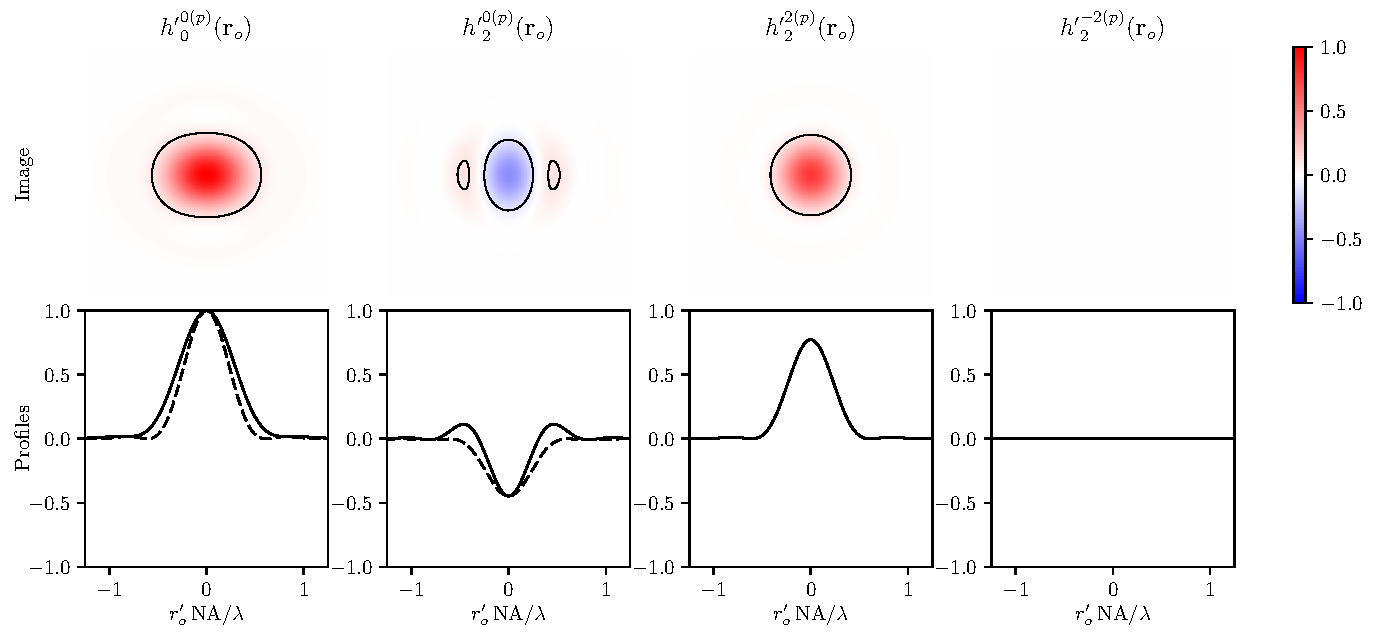
\includegraphics[width = 1.\textwidth]{../calculations/psfs0.pdf}
   \caption{Spatio-angular point spread function for a single-view fluorescence
     microscope with $\text{NA}=0.8$, $n_o=1.33$ and an $\mh{x}$-oriented
     polarizer under the paraxial approximation. \textbf{Columns:} Each term of
     the spatio-angular point spread function. \textbf{Row 1:} Images of each
     term with contours at $\pm 0.1$ and \textbf{Row 2:} horizontal (solid) and
     vertical (dashed) profiles through each term. The ${h'}_0^0$ and ${h'}_2^0$
     terms have a $\cos^2\phi_o$ dependence, so two profiles are sufficient to
     characterize their images. The ${h'}_2^2$ and ${h'}_2^{-2}$ terms are
     radially symmetric, so one profile is sufficient.}
   \label{fig:psf}
\end{figure}

The spatio-angular point spread function for a fluorescence microscope with a
polarized detection path has four terms---see Figures \ref{fig:psf} and \ref{fig:psf2} for plots.
The ${h'}_0^0$ and ${h'}_0^2$ terms are familiar from the unpolarized case, but
now they have an extra factor of $(\ro{}'\cdot\mh{p}_d)^2$ that accounts for the
polarizer and breaks radial symmetry. Notice that if we average over all
polarizer orientations then $(\ro{}'\cdot\mh{p}_d)^2 \rightarrow 1/2$, and we
recover the spatio-angular point spread function for a microscope without a
detection polarizer.

One of the interesting predictions of the polarized spatio-angular point spread
function is the elongated point spread function in the ${h'}_0^0$ term (which
corresponds to a physically realizable uniform distribution of dipoles). The
long axis of the point spread function is parallel with the transmission axis of
the polarizing filter---this is not an intuitive result. If we applied the usual
reasoning for the width of point spread functions---broader distributions of
intensity in the back focal plane cause narrower point spread functions---we
would predict that the point spread function for the ${h'}_0^0$ term would be
elongated perpendicular to the transmission axis of the polarizer. This
reasoning fails because we need to add the intensities at the detector, not at
the back focal plane.

The ${h'}_2^2$ and ${h'}_2^{-2}$ terms are only non-zero when a polarizing
filter is in the detection path. These terms correspond to distributions of
fluorophores with positive and negative fluorophores near the transverse plane
only. Without a polarizer, the ``intensity contributions'' from the positive and
negative fluorophores cancel, and we have no contribution from these
distributions. With a polarizer, the intensity contribution from the positive or
negative fluorophores dominate, and we end up with a rotationally symmetric
contribution to the point spread function.  

It's interesting to compare polarizing filters with phase and amplitude filters.
Adding a phase filter can extend the band limit of a microscope to measure new
information about the object without blocking any photons. For example, cubic
phase masks and microlens arrays can increase the axial band limit of a
microscope. All lenses can be considered as phase filters, so it's almost
obvious that phase filters can increase the band limit of an imaging system.
Amplitude filters, on the other hand, cannot extend the band limit of a
microscope. Amplitude filters can change the contrast for different spatial
frequencies by blocking photons, but they do not allow new information to be
measured. Polarizing filters share properties with phase and amplitude
filters---they block photons \textbf{and} extend the angular band limit of the
microscope. 

\begin{figure}[ht]
 \captionsetup{width=1.0\linewidth}
 \centering
   \centering
   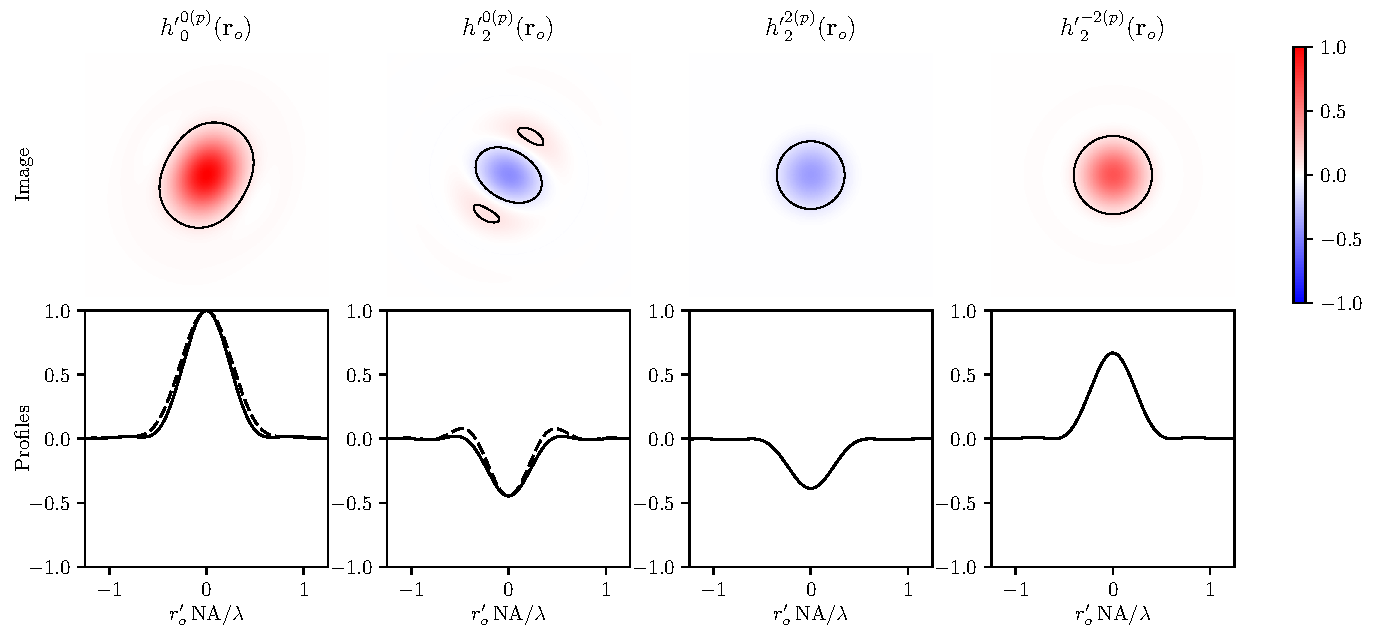
\includegraphics[width = 1.\textwidth]{../calculations/psfsp3.pdf}
   \caption{Spatio-angular point spread function for a single-view fluorescence
     microscope with $\text{NA}=0.8$, $n_o=1.33$ and an
     ($\mh{x}/2 + \sqrt{3}\mh{y}/2$)-oriented polarizer under the paraxial
     approximation. \textbf{Columns:} Each term of the spatio-angular point
     spread function. \textbf{Row 1:} Images of each term with contours at
     $\pm 0.1$ and \textbf{Row 2:} horizontal (solid) and vertical (dashed)
     profiles through each term. The ${h'}_0^0$ and ${h'}_2^0$ terms have a
     $\cos^2\phi_o$ dependence, so two profiles are sufficient to characterize
     their images. The ${h'}_2^2$ and ${h'}_2^{-2}$ terms are radially
     symmetric, so one profile is sufficient.}
   \label{fig:psf2}
\end{figure}

To find the transfer function we need to calculate the Fourier transform of the
point spread function. We can use the following Fourier transforms that we
evaluated in the previous notes
\begin{align}
\mathcal{F}_2\left\{{a^{(p)}}^2(r_o')\right\} &= 8\left[\arccos\left(\frac{\nu}{2\nu_o}\right) - \frac{\nu}{2\nu_o}\sqrt{1 - \left(\frac{\nu}{2\nu_o}\right)^2}\right]\Pi\left(\frac{\nu}{2\nu_o}\right),\\
\mathcal{F}_2\left\{{b^{(p)}}^2(r_o')\cos^2\phi'_o\right\} &= 4\left(\frac{\text{NA}}{n_o}\right)^2\Bigg[\arccos\left(\frac{\nu}{2\nu_o}\right) - \frac{1}{3}\left[5 - 2\left(\frac{\nu}{2\nu_o}\right)^2\right]\frac{\nu}{2\nu_o} \sqrt{1 - \left(\frac{\nu}{2\nu_o}\right)^2}\nonumber\\ &\hspace{17em} - \frac{8}{3}\cos^2\phi_\nu\frac{\nu}{2\nu_o}\sqrt[3]{1 - \left(\frac{\nu}{2\nu_o}\right)}\Bigg]\Pi\left(\frac{\nu}{2\nu_o}\right).              
\end{align}

Applying these results and normalizing gives the spatio-angular transfer function for
a fluorescence microscope with a polarizer along the detection path
\begin{align}
    H_m^{l(p)}(\bs{\nu}; \mh{p}_d) &= {H}_0^{0(p)}(\bs{\nu})\delta(l, m) + {H}_2^{0(p)}(\bs{\nu})\delta(l-2, m) + {H}_2^{2(p)}(\nu)\delta(l-2, m-2) + {H}_2^{-2(p)}(\nu)\delta(l-2, m+2),
\end{align}
where
\begin{align}
  {H}_0^{0(p)}(\bs{\nu}; \mh{p}_d) &\equiv \frac{1}{1 + (\text{NA}/n_o)^2}\left[{A^{(p)}}(\nu) + 2{B^{(p)}}(\nu) + 2{C^{(p)}}(\nu)\left\{2(\mh{\bs{\nu}}\cdot\mh{p}_d)^2 - 1\right\}\right],\\
  {H}_2^{0(p)}(\bs{\nu}; \mh{p}_d) &\equiv \frac{1}{\sqrt{5}[1 + (\text{NA}/n_o)^2]}\left[-{A^{(p)}}(\nu) + 4{B^{(p)}}(\nu) + 4{C^{(p)}}(\nu)\left\{2(\mh{\bs{\nu}}\cdot\mh{p}_d)^2 - 1\right\}\right],\\
  {H}_2^{2(p)}(\nu; \mh{p}_d) &\equiv \sqrt{\frac{3}{5}}\frac{1}{[1 + (\text{NA}/n_o)^2]}{A^{(p)}}(\nu)\left[(\mh{\bs{\nu}}\cdot\mh{x})^2 - (\mh{\bs{\nu}}\cdot\mh{y})^2\right],\\
  {H}_2^{-2(p)}(\nu; \mh{p}_d) &\equiv -2\sqrt{\frac{3}{5}}\frac{1}{[1 + (\text{NA}/n_o)^2]}{A^{(p)}}(\nu)(\mh{\bs{\nu}}\cdot\mh{x})(\mh{\bs{\nu}}\cdot\mh{y}),
\end{align}
and
\begin{align}
  {A}^{(p)}(\nu) &\equiv \frac{2}{\pi}\left[\arccos\left(\frac{\nu}{2\nu_o}\right) - \frac{\nu}{2\nu_o}\sqrt{1 - \left(\frac{\nu}{2\nu_o}\right)^2}\right]\Pi\left(\frac{\nu}{2\nu_o}\right),\\
  B^{(p)}(\nu) &\equiv \frac{1}{\pi}\left(\frac{\text{NA}}{n_o}\right)^2\left[\arccos\left(\frac{\nu}{2\nu_o}\right) - \left[3 - 2\left(\frac{\nu}{2\nu_o}\right)^2\right]\frac{\nu}{2\nu_o} \sqrt{1 - \left(\frac{\nu}{2\nu_o}\right)^2}\right]\Pi\left(\frac{\nu}{2\nu_o}\right),\\
  C^{(p)}(\nu) &\equiv \frac{1}{\pi}\left(\frac{\text{NA}}{n_o}\right)^2\left[-\frac{4}{3}\frac{\nu}{2\nu_o} \sqrt[3]{1 - \left(\frac{\nu}{2\nu_o}\right)^2}\right]\Pi\left(\frac{\nu}{2\nu_o}\right).                 
\end{align}

Figures \ref{fig:otf} and \ref{fig:otf2} show plots of the spatio-angular OTF
for two different polarizer orientations. Notice that the polarizer does not
change the spatial band limit of the microscope, but it does change the contrast
at high frequencies. If we use the cutoff frequency as a resolution criterion,
we would conclude that polarizers do not change the spatial resolution of our
microscope. However, if we use a spatial-domain resolution criteria like the
Rayleigh or Sparrow criteria, then we would conclude that adding a polarizer
improves the spatial resolution in the direction perpendicular to the polarizer.

Notice that the $H_0^0$ term in Figure \ref{fig:otf} is negative for spatial
frequencies near the cutoff frequency parallel to the polarizer transmission
axis. This means that we expect to see a contrast inversion for angularly
uniform distributions of dipoles when the spatial frequency pattern is parallel
to the polarizer transmission axis. In the spatial domain, this contrast
inversion is caused by the elongation of the point spread function. The point
spread function is wide enough that three fluorescent points spaced near the
cutoff frequency give an intensity minimum that reports the position of the
central fluorescent point---see Figure \ref{fig:psfmin}.

\begin{figure}[H]
 \captionsetup{width=1.0\linewidth}
 \centering
   \centering
   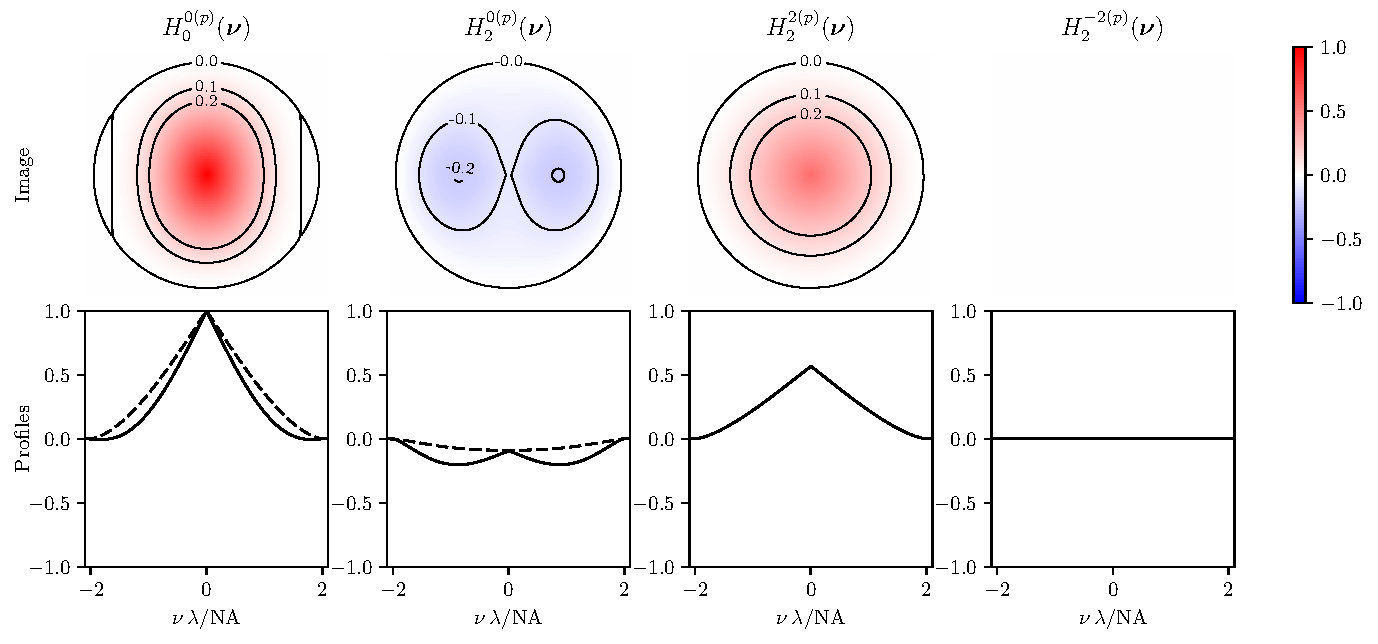
\includegraphics[width = 1.\textwidth]{../calculations/otfs0.pdf}
   \caption{Spatio-angular orientation transfer function for a single-view
     fluorescence microscope with $\text{NA}=0.8$, $n_o=1.33$ and an
     $\mh{x}$-oriented polarizer under the paraxial approximation.
     \textbf{Columns:} Each term of the spatio-angular optical transfer
     function. \textbf{Row 1:} Images of each term and \textbf{Row 2:}
     horizontal (solid) and vertical (dashed) profiles through each term.}
   \label{fig:otf}
\end{figure}


\begin{figure}[H]
 \captionsetup{width=1.0\linewidth}
 \centering
   \centering
   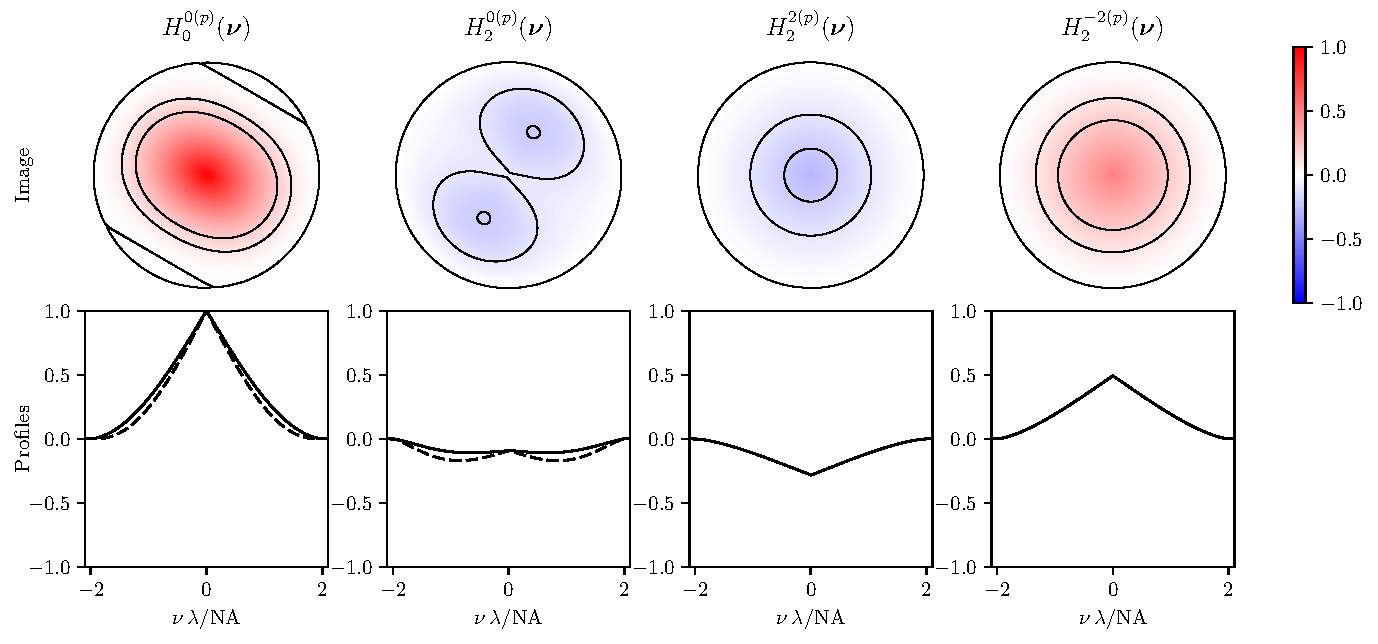
\includegraphics[width = 1.\textwidth]{../calculations/otfs3.pdf}
   \caption{Spatio-angular orientation transfer function for a single-view
     fluorescence microscope with $\text{NA}=0.8$, $n_o=1.33$ and an
     ($\mh{x}/2 + \sqrt{3}\mh{y}/2$)-oriented polarizer under the paraxial
     approximation. \textbf{Columns:} Each term of the spatio-angular optical
     transfer function. \textbf{Row 1:} Images of each term and \textbf{Row 2:}
     horizontal (solid), and vertical (dashed) profiles through each term.}
   \label{fig:otf2}
\end{figure}

\begin{figure}[H]
 \captionsetup{width=1.0\linewidth}
 \centering
   \centering
   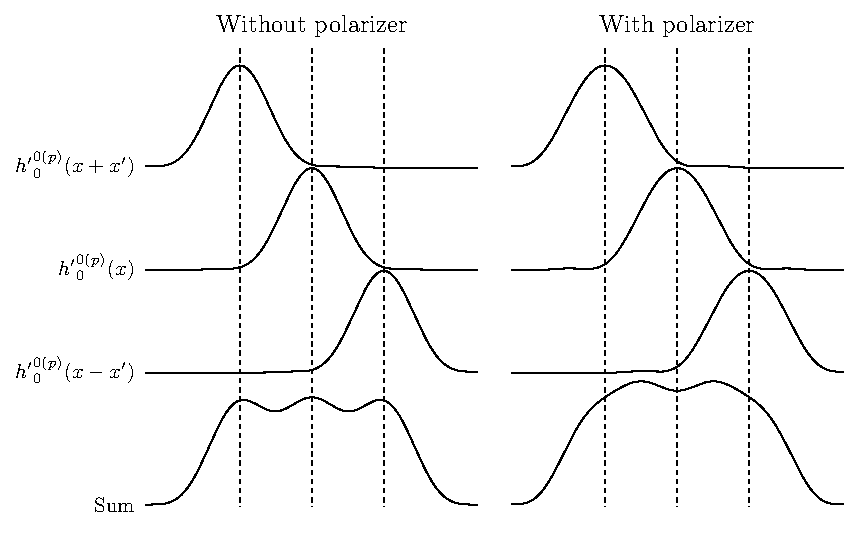
\includegraphics[width = 0.8\textwidth]{../calculations/psf-min.pdf}
   \caption{A polarizer creates a contrast inversion for uniformly distributed
     dipoles at high spatial frequencies along the direction parallel to the
     polarizer transmission axis. \textbf{Column 1:} Without a polarizer, three
     point sources with an angularly uniform distribution create an intensity
     pattern with three distinct peaks---the peaks report the position of the
     point sources. \textbf{Column 2:} With a polarizer, the point sources
     create an intensity pattern with two central peaks---the valley reports the
     position of the central point source. All of the sources in the figures are
     ``resolvable'' in the sense that they are spaced at a distance greater than
     the inverse of the cutoff frequency. This figure demonstrates contrast
     inversion at high spatial frequencies parallel to the polarizer
     transmission axis. }
   \label{fig:psfmin}
\end{figure}


% \begin{equation}
%   \begin{split}
%   h(\rd{}', \so{}; \mh{p}_d) \propto &\left(a^2(r_d') + 2b^2(r_d') + c^2(r_d')\right)y_0^0(\so{}) -\frac{2\sqrt{15}}{5}a(r_d')c(r_d')\sin(2\phi_d')y_2^{-2}(\so{})\\ &+ \frac{1}{\sqrt{5}}\left(-a^2(r_d') + 4b^2(r_d') - c^2(r_d')\right)y_2^{0}(\so{}) +\frac{2\sqrt{15}}{5}a(r_d')c(r_d')\cos(2\phi_d')y_2^{2}(\so{}). \label{eq:kerna}
% \end{split}
% \end{equation}

\appendix
\section{Rotation of spherical harmonics} \label{sec:sh} Given a spherical
function and its spherical harmonic coefficients $c_j$ (where $j$ is a single
index over the spherical harmonics), the spherical harmonic coefficients of the
rotated function $c'_i$ can be computed with the linear transformation
\begin{align}
  c_i' = \sum_j M_{ij}c_j, 
\end{align}
where the elements of the linear transformation can be computed with
\begin{align}
  M_{ij} = \int_{\mathbb{S}^2} d\so{}\, y_j(\mathbf{R}\so{})y_i(\so{}), 
\end{align}
where $\mathbf{R}$ is the rotation matrix that maps the original function to the
rotated function \cite{kautz2002}. If we assemble the elements of the linear transformation into
a matrix $\mathbf{M}$, then the matrix is block sparse
\begin{align}
  \mathbf{M} =
  \begin{bmatrix}[c|ccc|cccccc]    
    1&0&0&0&0&0&0&0&0&\cdots\\ \hline
    0&\mathbf{X}&\mathbf{X}&\mathbf{X}&0&0&0&0&0&\cdots\\
    0&\mathbf{X}&\mathbf{X}&\mathbf{X}&0&0&0&0&0&\cdots\\
    0&\mathbf{X}&\mathbf{X}&\mathbf{X}&0&0&0&0&0&\cdots\\ \hline
    0&0&0&0&\mathbf{X}&\mathbf{X}&\mathbf{X}&\mathbf{X}&\mathbf{X}&\cdots\\
    0&0&0&0&\mathbf{X}&\mathbf{X}&\mathbf{X}&\mathbf{X}&\mathbf{X}&\cdots\\
    0&0&0&0&\mathbf{X}&\mathbf{X}&\mathbf{X}&\mathbf{X}&\mathbf{X}&\cdots\\
    0&0&0&0&\mathbf{X}&\mathbf{X}&\mathbf{X}&\mathbf{X}&\mathbf{X}&\cdots\\
    0&0&0&0&\mathbf{X}&\mathbf{X}&\mathbf{X}&\mathbf{X}&\mathbf{X}&\cdots\\    
    \vdots&\vdots&\vdots&\vdots&\vdots&\vdots&\vdots&\vdots&\vdots&\ddots\\        
  \end{bmatrix}.
\end{align}
This means the spherical harmonic coefficients from each band transform
independently from the other bands.

To efficiently find the point spread functions and transfer functions for the
diSPIM we will compute the spherical harmonic coefficient transformation matrix
for a rotation that maps the $\mh{z}$ axis to the $\mh{x}$. The rotation matrix is
given by
\begin{align}
  \mb{R}_{\mh{z}\rightarrow\mh{x}} =
  \begin{bmatrix}
    0&0&1\\
    0&1&0\\
    -1&0&0    
  \end{bmatrix}, 
\end{align}
and the spherical harmonic coefficient transformation matrix is given by
\begin{align}
  \mathbf{M}_{\mh{z}\rightarrow\mh{x}} =
  \begin{bmatrix}[c|ccc|cccccc]
    1&0&0&0&0&0&0&0&0&\cdots\\ \hline 
    0&0&0&1&0&0&0&0&0&\cdots\\
    0&0&1&0&0&0&0&0&0&\cdots\\
    0&-1&0&0&0&0&0&0&0&\cdots\\ \hline 
    0&0&0&0&-1/2&0&0&\sqrt{3}/2&0&\cdots\\
    0&0&0&0&0&-1&0&0&0&\cdots\\
    0&0&0&0&0&0&0&0&-1&\cdots\\
    0&0&0&0&\sqrt{3}/{2}&0&0&1/2&0&\cdots\\
    0&0&0&0&0&0&1&0&0&\cdots\\    
    \vdots&\vdots&\vdots&\vdots&\vdots&\vdots&\vdots&\vdots&\vdots&\ddots\\        
  \end{bmatrix},
\end{align}
when the matrix elements are ordered as
$[y_0^0 | y_1^1, y_1^{-1}, y_1^0 | y_2^0, y_2^1, y_2^{-1}, y_2^2, y_2^{-2}]$.
For more complicated transformations (higher order coefficients or arbitrary
rotations) we can use recurrence relations to find the spherical harmonic
coefficient transformation matrix \cite{ivanic1996}.

\bibliography{report}{}
\bibliographystyle{unsrt}

\end{document}
